\documentclass[a4paper,12pt]{article}
\usepackage[utf8]{inputenc}
\usepackage[spanish]{babel}
\usepackage{xcolor}
\usepackage{geometry}
\usepackage{tikz}
\usepackage{lmodern}
\usepackage{titling}
\usepackage{amsmath, amssymb, amsthm}
\usepackage{enumitem}
\usepackage{graphicx}
\usepackage{titlesec}

\geometry{left=2.5cm, right=2.5cm, top=3cm, bottom=3cm}
\definecolor{azulPastel}{RGB}{173, 216, 230}

\begin{document}

\begin{titlepage}
    \thispagestyle{empty}
    \begin{tikzpicture}[remember picture, overlay]
        \fill[azulPastel] (current page.north west) rectangle ([yshift=-2cm]current page.north east);
        \fill[azulPastel] (current page.south west) rectangle ([yshift=2cm]current page.south east);
    \end{tikzpicture}

    \vspace*{3.5cm}
    \begin{center}
        {\scshape\LARGE Universidad de Málaga\par}
        \vspace{0.8cm}
        {\Large\bfseries Doble Grado en Ingeniería Informática y Matemáticas\par}
        \vspace{2.5cm}
        {\Huge\bfseries \textsc{K-COLOR es NP-completo}\par}
        \vspace{1cm}
        {\large\itshape Estudio de la reducción desde 3-SAT utilizando gadgets\par}
        \vspace{3.5cm}
        {\Large\textbf{Juan Elias Lara Soto}\par}
        \vspace{0.5cm}
        {\normalsize 2 de mayo de 2025\par}
    \end{center}
\end{titlepage}

\cleardoublepage  % Asegura que el índice empiece en página nueva
\section*{Índice}
\vspace{1em}

\begin{enumerate}
  \item \textbf{Definición del problema como lenguaje}
  \begin{enumerate}
    \item[1.1)] Ejemplo válido
    \item[1.2)] Ejemplo inválido
    \item[1.3)] Aplicaciones del problema
  \end{enumerate}
  
  \item \textbf{Demostración de que el problema es NP-completo}
  \begin{enumerate}
    \item[2.1)] El problema pertenece a NP
    \item[2.2)] Reducción desde un problema NP-completo
    \begin{enumerate}
      \item[a)] Descripción del problema fuente
      \item[b)] Ejemplo 
      \item [c)] Campo de aplicación del problema fuente
      \item[d)] Construcción del gadget con ejemplos
      \begin{itemize}
        \item Ejemplo válido
        \item Ejemplo inválido
      \end{itemize}
      \item[e)] Demostración de la doble implicación
      \begin{itemize}
        \item Si $\varphi$ es satisfacible, entonces el grafo es $k$-coloreable
        \item Si el grafo es $k$-coloreable, entonces $\varphi$ es satisfacible
      \end{itemize}
      \item[f)] Tiempo polinómico de la transformación
    \end{enumerate}
  \end{enumerate}

  \item \textbf{Preguntas sobre el ejercicio resuelto}
  \begin{enumerate}
   
  \end{enumerate}

  \item \textbf{Referencias bibliográficas}
\end{enumerate}

\newpage























\section{Definir el problema en forma de lenguaje}

Un \emph{coloreado} de un grafo es una asignación de colores a sus nodos de forma que ningún par de nodos adyacentes tenga el mismo color.

Sea el lenguaje:
\[
\text{3COLOR} = \{\langle G \rangle \mid G \text{ es coloreable con 3 colores} \}.
\]
Demuéstrese que \textbf{3COLOR} es NP-completo.

\vspace{1em}
Además, dado un número natural \(k \geq 3\), definimos el lenguaje generalizado:
\[
\begin{aligned}
k\text{-COLOR} = \big\{\, \langle G \rangle \;\big|\;\, &G \text{ es un grafo y es posible colorear sus nodos con } k \text{ colores} \\
&\text{de modo que ningún par de nodos adyacentes comparta color} \,\big\}.
\end{aligned}
\]

Demuéstrese que el problema \(k\text{-COLOR}\) es \textbf{NP-completo} para todo \(k \geq 3\).


\subsection{Ejemplo válido}
Grafo \( G_1 = (\{A, B, C\}, \{(A,B), (B,C), (A,C)\}) \): un triángulo completamente conectado que puede colorearse con tres colores distintos, uno por nodo.

\begin{center}
\begin{tikzpicture}[every node/.style={circle, draw, minimum size=1cm, font=\small}]
  \definecolor{verdeSuave}{RGB}{0,100,0}
  \definecolor{amarilloSuave}{RGB}{204,153,0}
  \definecolor{rojoSuave}{RGB}{200,0,0}

  \node[draw=verdeSuave, fill=verdeSuave!20] (A) at (0,0) {A};     
  \node[draw=amarilloSuave, fill=amarilloSuave!20] (B) at (2,0) {B};  
  \node[draw=rojoSuave, fill=rojoSuave!20] (C) at (1,1.7) {C};    

  \draw (A) -- (B) -- (C) -- (A);
\end{tikzpicture}
\end{center}

\subsection{Ejemplo inválido}
\[
\begin{aligned}
\text{Grafo } G_2 = (\{A, B, C, D, E\}, \{ &(A,B), (A,C), (A,D), (A,E), \\
&(B,C), (B,D), (B,E), (C,D), (C,E), (D,E) \}) \\
\end{aligned}

G2 está totalmente conectado con cinco nodos. No puede colorearse con solo tres colores sin conflictos.
\]


\begin{center}
\begin{tikzpicture}[every node/.style={circle, draw, minimum size=1cm, font=\small}]
  \definecolor{rojoSuave}{RGB}{200,0,0}
  \definecolor{azulSuave}{RGB}{30,144,255}
  \definecolor{verdeSuave}{RGB}{0,100,0}

  \node[draw=rojoSuave]   (A) at (90:2)   {A};   
  \node[draw=azulSuave]   (B) at (162:2)  {B};   
  \node[draw=verdeSuave]  (C) at (234:2)  {C};   
  \node[draw=rojoSuave]   (D) at (306:2)  {D};   
  \node[draw=azulSuave]   (E) at (18:2)   {E};   

  \draw[thick] (A) -- (B);
  \draw[thick] (A) -- (C);
  \draw[thick, red, line width=1.2pt] (A) -- (D); 
  \draw[thick] (A) -- (E);
  \draw[thick] (B) -- (C);
  \draw[thick] (B) -- (D);
  \draw[thick, red, line width=1.2pt] (B) -- (E); 
  \draw[thick] (C) -- (D);
  \draw[thick] (C) -- (E);
  \draw[thick] (D) -- (E);
\end{tikzpicture}
\end{center}

\subsection{ Aplicaciones de \texttt{3-COLOR} y \(k\)-COLOR (\(k > 3\))}
\begin{itemize}
  \item \textbf{Planificación de horarios y asignación de recursos:} En la programación de horarios escolares o universitarios, se puede modelar cada clase como un nodo en un grafo, y se conectan con una arista si comparten estudiantes o profesores. Una coloración adecuada asigna diferentes horarios (colores) a clases que no pueden ocurrir simultáneamente, minimizando conflictos.

  \item \textbf{Asignación de frecuencias en redes inalámbricas:} En telecomunicaciones, las estaciones base que están geográficamente cercanas deben operar en diferentes frecuencias para evitar interferencias. Modelando cada estación como un nodo y conectando aquellas que están dentro del rango de interferencia, una coloración del grafo asegura una asignación eficiente de frecuencias.

  \item \textbf{Diseño de circuitos electrónicos (VLSI):} En el diseño de circuitos integrados, componentes que no deben activarse simultáneamente se representan como nodos conectados. Una coloración adecuada ayuda a organizar las señales de control y minimizar interferencias, optimizando el rendimiento del circuito.

  \item \textbf{Coloración de mapas:} Aunque el Teorema de los Cuatro Colores establece que cualquier mapa plano puede colorearse con cuatro colores sin que regiones adyacentes compartan color, en mapas más complejos o en representaciones tridimensionales, puede requerirse más de cuatro colores. La coloración de grafos ayuda a determinar el número mínimo de colores necesarios para tales mapas.

  \item \textbf{Programación de tareas en sistemas operativos:} En la asignación de procesos a recursos compartidos, como CPUs o impresoras, se puede modelar cada proceso como un nodo y conectar aquellos que compiten por el mismo recurso. Una coloración del grafo asegura que procesos que requieren el mismo recurso no se ejecuten simultáneamente, evitando conflictos y mejorando la eficiencia del sistema.
\end{itemize}




\section{Prueba de que el problema es NP-Completo}

\subsection{Pertenencia a la clase NP}


\section*{Demostración 1: \( \text{3-COLOR} \in \text{NP} \)}

Para demostrar que el problema 3-COLOR pertenece a la clase NP, basta con proporcionar una forma de certificado y un algoritmo verificador que pueda validarlo en tiempo polinómico.

\begin{itemize}
    \item El \textbf{certificado} consiste en una asignación de uno de los tres colores posibles a cada vértice del grafo, de modo que ningún par de vértices conectados comparta el mismo color.
\end{itemize}

El \textbf{verificador} recibe como entrada un grafo \( G = (V, E) \) y una asignación de colores \( c \) y debe comprobar si se trata de una 3-coloración válida. Para ello, realiza las siguientes comprobaciones:

\begin{itemize}
    \item Recorre cada arista \( e = \{u, v\} \in E \), y verifica que los colores asignados a los extremos \( u \) y \( v \) son distintos.
    \item Si todas las aristas conectan vértices con colores diferentes, se acepta la certificación; en caso contrario, se rechaza.
\end{itemize}

Este procedimiento puede llevarse a cabo en tiempo polinómico:

\begin{itemize}[label=--]
    \item \( O(|E|) \) para recorrer las aristas del grafo.
    \item \( O(1) \) para verificar que los colores de los dos extremos de cada arista son distintos.
\end{itemize}

Dado que la verificación completa puede realizarse en \( O(n^2) \) como máximo, ya que el número de aristas como máximo en un grafo sera de \( n^2 \), concluimos que el problema cumple con las condiciones para pertenecer a NP.

\[
\Rightarrow \textbf{3-COLOR} \in \textbf{NP}
\]

\subsection{Reducción desde 3SAT}

\subsubsection{Descripción del problema fuente}

El problema \textbf{3-SAT} (abreviatura de \emph{3-Satisfiability}) es un problema de decisión en lógica proposicional. Se formula de la siguiente manera:

Dada una fórmula booleana $\varphi$ en \textbf{forma normal conjuntiva} (CNF), donde cada cláusula contiene exactamente \textbf{tres literales}, se pregunta:

\begin{center}
\emph{¿Existe una asignación de valores de verdad a las variables de $\varphi$ que haga verdadera toda la fórmula?}
\end{center}

Una fórmula está en forma CNF si es una conjunción (operación lógica AND) de cláusulas, y cada cláusula es una disyunción (operación lógica OR) de literales (variables o negaciones de variables).

Formalmente, una instancia de 3-SAT tiene la forma:
\[
\varphi = (l_{1,1} \lor l_{1,2} \lor l_{1,3}) \land (l_{2,1} \lor l_{2,2} \lor l_{2,3}) \land \dots \land (l_{m,1} \lor l_{m,2} \lor l_{m,3})
\]
donde cada literal $l_{i,j}$ es una variable proposicional $x_k$ o su negación $\neg x_k$.

\subsubsection{Ejemplo}

Considérese la fórmula:
\[
\varphi = (x_1 \lor \neg x_2 \lor x_3) \land (\neg x_1 \lor x_2 \lor x_4) \land (\neg x_3 \lor \neg x_4 \lor x_2)
\]

Una posible asignación que satisface la fórmula es:
\[
x_1 = \text{TRUE}, \quad x_2 = \text{TRUE}, \quad x_3 = \text{FALSE}, \quad x_4 = \text{FALSE}
\]

Verificamos que con esta asignación, cada cláusula es verdadera:
\begin{itemize}
  \item $(x_1 \lor \neg x_2 \lor x_3) = \text{TRUE} \lor \text{FALSE} \lor \text{FALSE} = \text{TRUE}$
  \item $(\neg x_1 \lor x_2 \lor x_4) = \text{FALSE} \lor \text{TRUE} \lor \text{FALSE} = \text{TRUE}$
  \item $(\neg x_3 \lor \neg x_4 \lor x_2) = \text{TRUE} \lor \text{TRUE} \lor \text{TRUE} = \text{TRUE}$
\end{itemize}

\subsubsection{Campo de aplicación}

El problema 3-SAT tiene aplicaciones fundamentales en muchas áreas de la informática y la inteligencia artificial. Un campo destacado es la \textbf{verificación de circuitos lógicos}:

En ingeniería de hardware y software, se necesita comprobar que un diseño lógico (como un circuito digital o un programa) cumple ciertas propiedades. Estas propiedades se pueden traducir en fórmulas booleanas. Verificar si existe una asignación que hace verdadera la fórmula equivale a comprobar si el diseño puede alcanzar un estado indeseado o si cumple una especificación.

También se aplica en:
\begin{itemize}
  \item Planificación automática en robótica e IA
  \item Resolución de problemas en lógica formal y juegos
  \item Teoría de bases de datos y restricciones
\end{itemize}

3-SAT es el prototipo de problema \textbf{NP-completo}, lo que significa que si se encontrara un algoritmo eficiente para resolverlo, se podría resolver eficientemente cualquier problema en la clase NP.



\subsubsection{ Construcción del gadeget con ejemplos}

Primero veremos que podemos reducir en tiempo polinómico el problema \textit{3SAT} a \textit{3-COLOR}, luego 3-COLOR es NP-Completo, y después daremos una generalización a \textit{k-COLOR} para cualquier $k > 3$.
\subsubsection*{ Explicación del gadget}

\paragraph{1. Gadget.} 
Comenzamos construyendo el gadget, el cual mediante una fórmula booleana en 3-CNF nos genere un grafo coloreable. Usamos la pista que nos proporciona el enunciado del ejercicio 38 del tema 7 del Spser. Se nos proponen los siguientes grafos:

\begin{itemize}
  \item \textbf{Palette gadget}: tres nodos conectados (T, F, R) que fijan los tres colores.
\begin{center}
\begin{tikzpicture}[every node/.style={circle, draw, minimum size=1cm, font=\small}]
  % Nodos del triángulo
  \node (F) at (0,2) {F};
  \node (T) at (-1,0) {T};
  \node (R) at (1,0) {};

  % Aristas del triángulo
  \draw (F) -- (T);
  \draw (F) -- (R);
  \draw (T) -- (R);

\end{tikzpicture}
\end{center}

  \item \textbf{Variable gadget}: dos nodos (\(+\), \(−\)) conectados a R.
\begin{center}
\begin{tikzpicture}[every node/.style={circle, draw, minimum size=1cm}, font=\small]

  % Nodos principales
  \node (A) at (0,0) {+};
  \node (B) at (2,0) {-};

  % Arista entre ellos
  \draw (A) -- (B);



\end{tikzpicture}
\end{center}

  \item \textbf{OR gadget}: simula disyunciones, con conexiones según la aparición del literal.
\begin{center}
\begin{tikzpicture}[every node/.style={circle, draw, minimum size=1cm, font=\small}]
  % Nodos
  \node (3) at (0,3) {3};     % Nodo superior
  \node (1) at (-1,1) {1};    % Centro izquierda
  \node (2) at (1,1) {2};     % Centro derecha
  \node (4) at (-1,-1) {4};    % Inferior izquierda
  \node (5) at (1,-1) {5};     % Inferior derecha

  % Aristas
  \draw (3) -- (1);
  \draw (3) -- (2);
  \draw (1) -- (2);
  \draw (1) -- (4);
  \draw (2) -- (5);
\end{tikzpicture}
\end{center}


Luego, sea $\varphi = C_1 \land C_2 \land \dots \land C_l$, una fórmula con $l$ cláusulas sobre el conjunto de variables booleanas $\{x_1, \dots, x_m\}$.

Construimos un grafo $G_\varphi$ (gadget) de la siguiente forma:
\begin{itemize}
  \item Usamos \textbf{dos variable-gadgets por cada variable} booleana $x_i$.
  \item Usamos \textbf{dos OR-gadgets por cada cláusula} $C_j$.
  \item Usamos \textbf{un único palette-gadget}.\\
\end{itemize}



\textbf{ELABORACIÓN DE LA REDUCCIÓN}

\paragraph{1.} A cada variable lógica le asociamos un \textbf{variable-gadget}, el cual etiquetamos con los símbolos \texttt{+} (variable true) y \texttt{-} (variable false). Este gadget se conecta directamente con el nodo \texttt{M} del palette, cuyos nombre de los nodos cobrarán sentido a posteriori (En este ejemplo, se representa únicamente un gadget de variable como si hubiera una sola variable en la fórmula.). 

\begin{center}
\begin{tikzpicture}[every node/.style={circle, draw, minimum size=1cm, font=\small}]
  % Palette-gadget
  \node (F) at (0,2) {F};
  \node (T) at (-1,0) {T};
  \node (M) at (1,0) {M};
  \draw (T) -- (F) -- (M) -- (T);

  % Variable-gadget
  \node (plus) at (3,0) {+};
  \node (minus) at (3,2) {-};
  \draw (plus) -- (minus);
  \draw (M) -- (plus);
  \draw (M) -- (minus);
\end{tikzpicture}
\end{center}
\paragraph{2.}1 A cada cláusula de la fórmula le corresponden dos \textbf{OR-gadgets}. En este paso, conectamos el nodo superior , esto es, el nodo 3 del primer OR-gadget, con el nodo \texttt{F} del palette definido previamente. Además, dicho nodo 3 también se conecta con el nodo \texttt{M}, cerrando así la parte superior de la estructura.

\begin{center}
\begin{tikzpicture}[every node/.style={circle, draw, minimum size=1cm, font=\small}]

  % Palette-gadget
  \node (F) at (0,0) {F};
  \node (T) at (-1,-2) {T};
  \node (M) at (1,-2) {M};
  \draw (T) -- (F) -- (M) -- (T);

  % Variable gadget
  \node (plus) at (3,-2) {+};
  \node (minus) at (3,0) {-};
  \draw (plus) -- (minus);
  \draw (M) -- (plus);
  \draw (M)--(minus);


  % OR-gadget
  \node (3) at (0,2) {3};
  \node (1) at (-1,3) {1};
  \node (2) at (1,3) {2};
  \node (4) at (-1,5) {4};
  \node (5) at (1,5) {5};

  \draw (3) -- (1);
  \draw (3) -- (2);
  \draw (1) -- (2);
  \draw (1) -- (4);
  \draw (2) -- (5);

  % Conexiones a F y M
  \draw (3) -- (F);
  \draw (3) -- (M);
\end{tikzpicture}
\end{center}

\paragraph{2.2} A continuación, reemplazamos uno de los nodos inferiores del primer OR-gadget por el nodo superior del segundo OR-gadget. Así se encadena el nuevo gadget a la estructura. En este proceso, el nodo \texttt{4} es eliminado y sustituido por el nuevo subgrafo.

\begin{center}
\begin{tikzpicture}[every node/.style={circle, draw, minimum size=1cm, font=\small}]
  % Primer OR-gadget (superior)
  \node (5a) at (2,5) {5};
  \node (1a) at (0,3) {1};
  \node (2a) at (2,3) {2};
  \node (3a) at (1,2) {3};

  \draw (2a) -- (5a);
  \draw (1a) -- (2a);
  \draw (3a) -- (1a);
  \draw (3a) -- (2a);

  % Segundo OR-gadget (conectado a 1a en lugar de 4)
  \node (5b) at (1,8) {5};
  \node (1b) at (-1,6) {1};
  \node (2b) at (1,6) {2};
  \node (3b) at (0,5) {3};
  \node (4b) at (-1,8) {4};
  
  \draw (1b) -- (4b);
  \draw (3b) -- (1b);
  \draw (3b) -- (2b);
  \draw (1b) -- (2b);
  \draw (2b) -- (5b);
  \draw (1a) -- (3b); % Conexión desde OR-gadget superior

  % Palette-gadget
  \node (F) at (0,0) {F};
  \node (T) at (-1,-2) {T};
  \node (M) at (1,-2) {M};
  \draw (T) -- (F) -- (M) -- (T);

  % Variable gadget
  \node (plus) at (3,-2) {+};
  \node (minus) at (3,0) {-};
  \draw (plus) -- (minus);
  \draw (M) -- (plus);
  \draw (M)--(minus);


  % Conexiones principales
  \draw (3a) -- (F);
  \draw (3a) -- (M);
\end{tikzpicture}
\end{center}
\textbf{3.} Ahora conectamos los nodos 4,5 y 5 con con el \textbf{variable-gadget} correspondiente. Si la cláusula incluye la variable $x_i$, se hace corresponder con el nodo \texttt{+} del variable-gadget asociado. Si en su lugar aparece $\neg x_i$, se vincula con el nodo \texttt{-}. Por ello el nodo 4 pasa a ser el mismo que - y el nodo 5 pasa a ser el mismo que mas.

En este dibujo, se ha representado una sola variable, y por tanto, un solo variable-gadget. Sin pérdida de generalidad, las aristas rojas y verdes podrían ser un ejemplo valido para el gadget correspondiente para una 3-CNF dada.

\begin{center}
\begin{tikzpicture}[
  every node/.style={circle, draw, minimum size=1cm, font=\small},
  identmas/.style={thick, draw=green!70!black},
  identmenos/.style={thick, draw=red}
]

  % OR-gadget superior
  \node (1a) at (0,3) {1};
  \node (2a) at (2,3) {2};
  \node (3a) at (1,2) {3};

  \draw (1a) -- (2a);
  \draw (1a) -- (3a);
  \draw (2a) -- (3a);

  % OR-gadget medio
  \node (1b) at (-1,8) {1};
  \node (2b) at (5,8) {2};
  \node (3b) at (2,5) {3};

  \draw (1b) -- (2b);
  \draw (1b) -- (3b);
  \draw (2b) -- (3b);
  \draw (1a) -- (3b);

  % Conexiones a gadget inferior
  \node (F) at (0,0) {F};
  \node (T) at (-1,-2) {T};
  \node (R) at (1,-2) {M};
  \draw (T) -- (F) -- (R) -- (T);

  % Variable-gadget
  \node (plus) at (3,-2) {+};
  \node (minus) at (3,0) {-};
  \draw (plus) -- (minus);
  \draw (R) -- (plus);
  \draw (M)--(minus);


  % Conexiones con F y R
  \draw (3a) -- (F);
  \draw (3a) -- (R);

  % Conexiones identificadas con colores
  \draw[identmenos] (1b) -- (minus);   % nodo 4 → -
  \draw (1b) -- (plus);   % nodo 4 → -
 \draw (2a) -- (minus);   % nodo 4 → -
  \draw (2b) -- (minus);   % nodo 4 → -
  \draw[identmas] (2a) -- (plus);      % nodo 5 → +
  \draw[identmas] (2b) -- (plus);      % nodo 5 → +

\end{tikzpicture}
\end{center}
\textbf{4.} Asignamos colores a los nodos del grafo según el \textit{palette-gadget}: T (\textcolor{green!50!black}{verde}), F (\textcolor{red}{rojo}) y M (\textcolor{brown}{marrón}).

Finalmente, debemos abordar el coloreado de los nodos en el grafo. Para ello, utilizamos las referencias proporcionadas por el \textit{Pallette-Gadget}, en el que los símbolos $T$, $F$ y $M$ representan colores distintos. 

Para cada variable, asignamos al nodo $+$ el color $T$ y al nodo $-$ el color $F$ en el \textit{Variable-Pallette}, siempre que dicha variable tome el valor verdadero en una asignación que satisfaga $\varphi$ (lo cual sucederá si $\varphi$ es satisfacible). En caso contrario (si $\varphi$ es insatisfacible, por ejemplo), invertimos esta asignación de colores.

Como cada cláusula posee al menos un literal que se evalúa como verdadero bajo una asignación satisfactoria, existirá al menos una entrada al \textit{OR-Gadget} que esté coloreada con $T$. Esto permite colorear adecuadamente los nodos del \textit{OR-Gadget} de forma que el nodo conectado al $F$ del \textit{Pallette-Gadget} no adopte el color rojo ($F$). En consecuencia, se obtiene una 3-coloración válida.

Por otro lado, si $\varphi$ no es satisfacible, todas las entradas al \textit{OR-Gadget} estarán coloreadas con $F$, lo que forzará a que el nodo vinculado al $F$ del \textit{Pallette-Gadget} adopte también el color $F$, lo que produce una coloración no válida.\\



\textbf{Ejemplo válido}

Consideremos el ejemplo más sencillo para poder ver con claridad las aristas del grafo y que no resulte imposible distinguirlas, este es, la fórmula booleana $\varphi = (x \lor x \lor x)$, que se encuentra en 3CNF.

La fórmula $\varphi$ resulta ser satisfacible, ya que, asignando a $x$ el valor verdadero, la cláusula queda satisfecha. Dado que únicamente consta de una cláusula y una variable, el proceso de construcción del grafo $G_\varphi$ se lleva a cabo exactamente como se explicó anteriormente.


\begin{center}
\begin{tikzpicture}[
  every node/.style={circle, draw, minimum size=1cm, font=\small},
  identmas/.style={thick, draw=black!70!black},
  identmenos/.style={thick, draw=black}
]

  % OR-gadget superior
  \node (1a) at (0,3) {1};
  \node (2a) at (2,3) {2};
  \node (3a) at (1,1) {3};

  \draw (1a) -- (2a);
  \draw (1a) -- (3a);
  \draw (2a) -- (3a);

  % OR-gadget medio
  \node (1b) at (1,6) {1};
  \node (2b) at (3,6) {2};
  \node (3b) at (2,5) {3};

  \draw (1b) -- (2b);
  \draw (1b) -- (3b);
  \draw (2b) -- (3b);
  \draw (1a) -- (3b);

  % Conexiones a gadget inferior
  \node (F) at (0,0) {F};
  \node (T) at (-1,-2) {T};
  \node (R) at (1,-2) {M};
  \draw (T) -- (F) -- (R) -- (T);

  % Variable-gadget
  \node (plus) at (5,-2) {+};
  \node (minus) at (2,0) {-};
  \draw (plus) -- (minus);
  \draw (R) -- (plus);
  \draw (M)--(minus);


  % Conexiones con F y R
  \draw (3a) -- (F);
  \draw (3a) -- (R);

  % Conexiones identificadas con colores
  \draw[identmenos] (1b) -- (plus);   % nodo 4 → -
  \draw[identmas] (2a) -- (plus);      % nodo 5 → +
  \draw[identmas] (2b) -- (plus);      % nodo 5 → +

\end{tikzpicture}
\end{center}

Tenemos que $\varphi$ es una formúla satisfacible, luego asignamos el color del nodo T a + y el color de F al nodo -. Luego, el nodo 3 que conecta con el nodo F ha de ser verde para que sea válida la coloración.
Teniendo en cuenta lo mencionado, coloreamos el grafo con una coloración válida.



  % OR-gadget superior
  \begin{center}
\begin{tikzpicture}[scale=1, every node/.style={scale=1, circle, draw, minimum size=0.8cm, font=\small}]
    
    % Definimos colores
    \definecolor{verdeT}{RGB}{0,128,0}  % Verde oscuro
    \definecolor{rojoF}{RGB}{255,0,0}   % Rojo brillante
    \definecolor{marronR}{RGB}{139,69,19} % Marrón oscuro
    
    % OR-gadget inferior
    \node[draw=marronR] (1a) at (0,3) {1};   % Color T
    \node[draw=rojoF] (2a) at (2,3) {2};  % Color R
    \node[draw=verdeT] (3a) at (1,2) {3};    % Color F
    
    \draw (1a) -- (2a);
    \draw (1a) -- (3a);
    \draw (2a) -- (3a);
    
    % OR-gadget medio
    \node[draw=marronR] (1b) at (1,6) {1};    % Color T
    \node[draw=rojoF] (2b) at (3,6) {2};   % Color R
    \node[draw=verdeT] (3b) at (2,5) {3};     % Color F
    
    \draw (1b) -- (2b);
    \draw (1b) -- (3b);
    \draw (2b) -- (3b);
    \draw (1a) -- (3b);
    
    % Conexiones a gadget inferior (PALLETTE-GADGET)
    \node[draw=rojoF] (F) at (0,0) {F};     % Color F
    \node[draw=verdeT] (T) at (-1,-2) {T};  % Color T
    \node[draw=marronR] (R) at (1,-2) {M};  % Color R
    
    \draw (T) -- (F) -- (R) -- (T);
    
    % Variable-gadget
    \node[draw=verdeT] (plus) at (5,-2) {+};  % Color T
    \node[draw=rojoF] (minus) at (2,0) {-};   % Color F
    
    \draw (plus) -- (minus);
    \draw (R) -- (plus);
    \draw (R) -- (minus);
    
    % Conexiones adicionales
    \draw (3a) -- (F);
    \draw (3a) -- (R);
    
    % Conexiones identificadas (usando estilos si quieres)
    \draw (1b) -- (plus);   % nodo 1a → -
    \draw (2a) -- (plus);    % nodo 2a → +
    \draw (2b) -- (plus);    % nodo 2b → +

\end{tikzpicture}
\end{center}
Se observa claramente, que es una 3-coloración válida, la cual se ha obtenido a partir de una fórmula satisfacible.\\

\textbf{Ejemplo inválido}

Consideremos ahora la formula 3-CNF insatisfacible más sencilla que se nos puede ocurrir: $\varphi = (x_1 \lor x_1 \lor x_1) \land (\lnot x_1 \lor \lnot x_1 \lor \lnot x_1)$. Esta fórmula posee una variable y dos cláusulas.

La fórmula $\varphi$ es insatisfacible, ya que, para cualquier asignación de valor de verdad a $x_1$, se requiere simultáneamente que $x_1$ y su negación sean verdaderos, lo cual es imposible. Por ejemplo, asignar el valor 1 a $x_1$ no logra satisfacer $\varphi$.

Dado que el número de cláusulas es dos y sólo se maneja una variable, el procedimiento de construcción del grafo $G_\varphi$ sigue la metodología descrita anteriormente, teniendo en cuenta que ahora se incorporarán dos gadgets tipo OR adicionales.


\begin{center}
\begin{tikzpicture}[every node/.style={circle, draw=black, minimum size=1cm, font=\small}]

% Pallette Gadget
\node (T) at (-6,-6) {T};
\node (F) at (-3,-4) {F};
\node (R) at (0,-6) {M};
\draw (T) -- (F) -- (R) -- (T);

% Variable Gadget
\node (plus) at (2,2) {+};
\node (minus) at (1,4) {-};
\draw (plus) -- (minus);

% OR-gadget izquierdo
\node (L1) at (-8, 6) {1};
\node (L2) at (-4, 6) {2};
\node (L3) at (-6, 4) {3};
\draw (L1) -- (L2) -- (L3) -- (L1);

% OR-gadget medio
\node (M1) at (-7,1) {1};
\node (M2) at (-3,1) {2};
\node (M3) at (-5, 0) {3};
\draw (M1) -- (M2) -- (M3) -- (M1);

% OR-gadget derecho
\node (R1) at (3, 6) {1};
\node (R2) at (7, 6) {2};
\node (R3) at (5, 4) {3};
\draw (R1) -- (R2) -- (R3) -- (R1);

% OR-gadget extremo derecho
\node (RR1) at (4,1) {1};
\node (RR2) at (6,1) {2};
\node (RR3) at (5, -1) {3};
\draw (RR1) -- (RR2) -- (RR3) -- (RR1);

% Conexiones adicionales con + y -
\draw (F) -- (M3);
\draw (F) -- (RR3);
\draw (R) -- (M3);
\draw (R) -- (minus);
\draw (R) -- (plus);
\draw (R) -- (RR3);

\draw (M2) -- (plus);
\draw (M1) -- (L3);

\draw (plus) -- (L1);
\draw (plus) -- (L2);

\draw (RR1) -- (R3);
\draw (RR2) -- (minus);
\draw (R2) -- (minus);
\draw (R1) -- (minus);

\end{tikzpicture}
\end{center}

Coloreamos el palette gadget y el variable gadget teniendo en cuenta que x1 igual a true hace falsa la fórmula booleana, luego - sera verde y + sera rojo. A partir de aqui coloreamos cada cláusula de forma independiente ya que cada cláusula por separado si que es satisfacible, luego, obtenemos la siguiente 3-coloración.



\begin{center}
\begin{tikzpicture}[every node/.style={circle, draw, minimum size=1cm, font=\small}]

% Definimos colores suaves para bordes
\definecolor{verdeBorde}{RGB}{0,120,0}
\definecolor{rojoBorde}{RGB}{180,0,0}
\definecolor{marronBorde}{RGB}{139,69,19}

% Pallette Gadget (más abajo y separado)
\node[draw=verdeBorde] (T) at (-6,-6) {T};
\node[draw=rojoBorde] (F) at (-3,-4) {F};
\node[draw=marronBorde] (R) at (0,-6) {M};
\draw (T) -- (F) -- (R) -- (T);

% Variable Gadget
\node[draw=rojoBorde] (plus) at (2,2) {+};
\node[draw=verdeBorde] (minus) at (1,4) {-};
\draw (plus) -- (minus);

% OR-gadget izquierdo
\node[draw=marronBorde] (L1) at (-8, 6) {1};
\node[draw=verdeBorde] (L2) at (-4, 6) {2};
\node[draw=rojoBorde] (L3) at (-6, 4) {3};
\draw (L1) -- (L2) -- (L3) -- (L1);

% OR-gadget medio
\node[draw=verdeBorde] (M1) at (-7,1) {1};
\node[draw=marronBorde] (M2) at (-3,1) {2};
\node[draw=rojoBorde] (M3) at (-5, 0) {3};
\draw (M1) -- (M2) -- (M3) -- (M1);

% OR-gadget derecho
\node[draw=rojoBorde] (R1) at (3, 6) {1};
\node[draw=marronBorde] (R2) at (7, 6) {2};
\node[draw=verdeBorde] (R3) at (5, 4) {3};
\draw (R1) -- (R2) -- (R3) -- (R1);

% OR-gadget extremo derecho
\node[draw=marronBorde] (RR1) at (4,1) {1};
\node[draw=rojoBorde] (RR2) at (6,1) {2};
\node[draw=verdeBorde] (RR3) at (5, -1) {3};
\draw (RR1) -- (RR2) -- (RR3) -- (RR1);

% Conexiones adicionales con + y -

% �� Arista destacada F -- M3 en amarillo y rojo
\draw[ultra thick, draw=red, double=yellow, double distance=1.5pt] (F) -- (M3);

% Resto de aristas
\draw (F) -- (RR3);
\draw (R) -- (M3);
\draw (R) -- (minus);
\draw (R) -- (plus);
\draw (R) -- (RR3);

\draw (M2) -- (plus);
\draw (M1) -- (L3);

\draw (plus) -- (L1);
\draw (plus) -- (L2);

\draw (RR1) -- (R3);
\draw (RR2) -- (minus);
\draw (R2) -- (minus);
\draw (R1) -- (minus);

\end{tikzpicture}
\end{center}



\textbf Observamos que, al realizar la coloración propuesta, el nodo \texttt{F} del \emph{palette gadget} y el nodo \texttt{3} del \emph{OR-gadget central} (asociado a la segunda cláusula) están unidos por una arista y, sin embargo, han sido coloreados con el mismo color (rojo). Esto viola la condición fundamental de una 3-coloración válida, que requiere que todo par de nodos adyacentes tengan colores distintos. Por tanto, esta coloración no es válida y refleja correctamente la insatisfacibilidad de la fórmula original.

\theoremstyle{plain}
\newtheorem{theorem}{Teorema}

\subsubsection{Demostracion de la doble implicación}
\textbf{Teorema: }
\textbf{3-COLOURING es NP-completo}


\textbf{Demostración}:  

\textbf{1. 3-COLOURING pertenece a NP.}

Ya lo hemos visto en este documento.






\textbf{2. 3-COLOURING es NP-hard.}

Para probar la NP-dificultad, se da una reducción polinomial desde 3-SAT a 3-COLOURING. Es decir, dada una instancia \( \varphi \) de 3-SAT, veremos que el gadget construido anteriormente 3-colorable si y solo si \( \varphi \) es satisfacible.

\textbf{Captura de cláusulas mediante gadgets OR.}

Para reflejar las cláusulas de \( \varphi \), se introduce un gadget OR para cada cláusula \( C_i = (a \lor b \lor c) \).

Este gadget conecta los literales \( a, b, c \) y tiene un nodo de salida que representa \( a \lor b \lor c \). El gadget se construye en dos etapas: primero se calcula \( a \lor b \), luego \((a \lor b) \lor c\).

El gadget satisface las siguientes propiedades:
\begin{enumerate}
    \item Si \( a \), \( b \) y \( c \) están coloreados con \( F \), entonces el nodo de salida debe estar coloreado también con \( F \), reflejando que la cláusula no está satisfecha.
    \item Si al menos uno de \( a \), \( b \) o \( c \) está coloreado con \( T \), entonces existe una 3-coloración válida del gadget en la que el nodo de salida se colorea con \( T \), reflejando que la cláusula sí está satisfecha.
\end{enumerate}

Una vez construidos todos los gadgets OR, cada nodo de salida se conecta a los vértices \( F \) y \( B \) del triángulo inicial.


\begin{figure}[h]
    \centering
    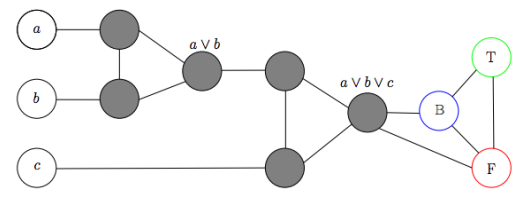
\includegraphics[width=0.5\linewidth]{image2.png}
    \caption{ Mouatadid 2014}
    \label{fig:enter-label}
\end{figure}
\textbf{Finalización de la prueba.}
\\
\textbf{(\( \Rightarrow \))} Supongamos que \( \varphi \) es satisfacible, y sea \( (x_1^*, x_2^*, \dots, x_n^*) \) una asignación satisfactoria.  
Coloreamos cada \( v_i \) con \( T \) si \( x_i^* = 1 \) y \( \overline{v}_i \) con \( F \); o viceversa si \( x_i^* = 0 \). Dado que cada cláusula \( C_i = (a \lor b \lor c) \) tiene al menos un literal verdadero, el correspondiente gadget OR puede ser 3-coloreado de modo que el nodo de salida esté coloreado \( T \), respetando la conexión a \( F \) y \( B \).

\textbf{(\( \Leftarrow \))} Supongamos ahora que \( G \) es 3-colorable.  
Definimos una asignación de valores de verdad de la siguiente forma: asignamos \( x_i = 1 \) si \( v_i \) tiene color \( T \), y \( x_i = 0 \) si \( \overline{v}_i \) tiene color \( T \).  
Si esta asignación no satisficiera \( \varphi \), existiría una cláusula \( C_i \) donde todos los literales fueran falsos, lo que implicaría que el nodo de salida del gadget OR estaría coloreado \( F \), en conflicto con su conexión al vértice \( F \) del triángulo, violando así la 3-colorabilidad.

Por tanto, \( \varphi \) es satisfacible si y solo si \( G \) es 3-colorable.
\subsubsection{Tiempo polinómico}

Vamos a justificar que tanto la construcción del grafo $G_\varphi$ como su proceso de 3-coloración se realizan en tiempo polinómico con respecto al tamaño de la entrada, es decir, el número de variables $n$ y de cláusulas $l$.

\textbf{Construcción del grafo $G_\varphi$}

La generación del grafo comienza con la creación de un único \emph{palette gadget}, que consta de un número fijo de nodos y aristas, por lo que su construcción requiere tiempo constante.

A continuación, para cada variable booleana de la fórmula, se incorpora un \emph{variable gadget}, el cual está compuesto por dos nodos conectados entre sí. Dado que el número de variables es $n$, el número total de nodos y aristas añadidos por este paso es proporcional a $n$.

Respecto a las cláusulas, cada una se representa mediante dos \emph{OR gadgets} modificados. Aunque la versión clásica contiene 8 nodos, en este caso se simplifican eliminando los dos nodos auxiliares finales, lo que deja 6 nodos y 7 aristas por cláusula. Como hay $l$ cláusulas, el total de nodos y aristas introducidos por este paso también es lineal respecto a $l$.

En resumen, el número total de operaciones necesarias para construir todos los gadgets del grafo es proporcional a $n + l$, lo cual implica una complejidad de construcción en tiempo $\mathcal{O}(n + l)$.

\textbf{Coloración en tres colores}

Una vez construido el grafo, se procede a su coloración utilizando tres colores. Este proceso consiste en recorrer todos los nodos y asignarles un color de acuerdo con las reglas establecidas por los gadgets construidos. Dado que el número de nodos y aristas es lineal en función de $n$ y $l$, y que cada operación de asignación de color puede realizarse en tiempo constante, el tiempo total de este proceso también es polinómico.

\textbf{Conclusión}

Tanto la generación del grafo $G_\varphi$ como su coloración bajo la restricción de 3 colores se realizan en tiempo polinómico respecto al tamaño de la fórmula de entrada. Por lo tanto, el método es computacionalmente eficiente en términos de complejidad temporal.




\subsubsection{Demostración de que \texorpdfstring{$k$}-COLOR es NP-completo para \texorpdfstring{$k \geq 3$}}

Consideramos el problema de decidir si un grafo puede colorearse utilizando a lo sumo $k$ colores, de modo que vértices adyacentes reciban colores distintos. Este problema, denominado \textsc{$k$-COLOR}, generaliza el conocido \textsc{3-COLOR}.

Es intuitivo pensar que si un grafo es 3-coloreable, también lo será para cualquier número mayor de colores, ya que bastará con emplear únicamente tres de los $k$ disponibles e ignorar los restantes. En este sentido, \textsc{3-COLOR} puede verse como un caso particular de \textsc{$k$-COLOR}.

Vamos a demostrar formalmente que \textsc{$k$-COLOR} es NP-completo para cualquier $k \geq 3$.

\textbf{Pertenencia a NP.} La verificación de una $k$-coloración consiste en comprobar que cada par de vértices adyacentes recibe colores distintos y que el total de colores utilizados no supera $k$. Usando un certificado análogo al que se utilizó para 3-color, existe un certificado con una asignación de colores a los vértices, esta comprobación puede realizarse en tiempo polinómico. Por tanto, \textsc{$k$-COLOR} pertenece a NP.

\textbf{Reducción desde \textsc{3-COLOR}.} Para demostrar la NP-completitud, basta construir una reducción polinómica desde \textsc{3-COLOR}, que ya sabemos que es NP-completo.

Dada una instancia $G$ del problema \textsc{3-COLOR}, construiremos un grafo $H$ tal que $G$ es 3-coloreable si y solo si $H$ es $k$-coloreable.

El grafo $H$ se obtiene de $G$ añadiendo un subgrafo completamente conexo (clique) con $k - 3$ nuevos vértices. A continuación, conectamos cada uno de estos nuevos vértices con todos los vértices del grafo $G$ original.

\textbf{Correctitud de la reducción.}
\begin{itemize}
    \item Si $G$ admite una 3-coloración válida, podemos extender esta coloración a $H$ asignando a los $k-3$ nuevos vértices colores distintos y distintos de los ya usados en $G$, lo cual es posible porque estos nuevos vértices forman una clique y están conectados a todo $G$.
    \item Si $G$ no es 3-coloreable, entonces para colorear $H$ necesitamos al menos $k-3$ colores sólo para los nuevos vértices, y no podremos asignar colores a $G$ usando únicamente los 3 colores restantes, ya que por hipótesis $G$ no es 3-coloreable. Por tanto, $H$ no será $k$-coloreable.
\end{itemize}

Este procedimiento de construcción es claramente polinómico en el tamaño de $G$, ya que sólo añade un número constante de vértices y aristas en función de $k$.

\textbf{Conclusión.} Hemos demostrado que \textsc{$k$-COLOR} pertenece a NP y que existe una reducción polinómica desde \textsc{3-COLOR}. Por tanto, se concluye que \textsc{$k$-COLOR} es NP-completo para todo $k \geq 3$.

\section{Preguntas tipo test sobre la reducción de 3-SAT a 3-COLOR}


\section*{Pregunta 1}

\textbf{¿Cómo se representa una variable negada (¬x) en el grafo construido a partir de una fórmula 3-CNF?}

\begin{enumerate}[label=\Alph*)]
    \item Conectando el nodo + del gadget de variable al OR-gadget
    \item Asignándole el mismo color que el nodo M
    \item {Conectando el nodo – del gadget de variable al OR-gadget} % Respuesta correcta
    \item Usando un gadget de cláusula adicional
\end{enumerate}

\section*{Pregunta 2}

\textbf{¿Cómo se asegura la correspondencia entre la satisfacibilidad de una fórmula y la 3-colorabilidad del grafo construido?}

\begin{enumerate}[label=\Alph*)]
    \item Cada cláusula se convierte en un triángulo coloreable
    \item {El gadget OR permite que al menos una entrada tenga color T si la cláusula es verdadera} % Respuesta correcta
    \item Los colores se asignan al azar para simular todas las asignaciones
    \item Si el grafo tiene ciclos, entonces la fórmula no es satisfacible
\end{enumerate}

\section*{Pregunta 3}

\textbf{¿Qué ocurre si una fórmula booleana es insatisfacible al aplicar la reducción a 3-COLOR?}

\begin{enumerate}[label=\Alph*)]
    \item El grafo resultante no tiene aristas
    \item La construcción del gadget falla
    \item {No existe una 3-coloración válida para el grafo} % Respuesta correcta
    \item El grafo se vuelve completamente conexo
\end{enumerate}



\section{Referencias bibliográficas}



Youssef Mouatadid. \textit{Gadget Reductions: 3-SAT to 3-COLOR}. Lecture notes, CSC373, University of Toronto, 2016.\\
\text{https://www.cs.toronto.edu/~lalla/373s16/notes/3col.pdf}

Kristin Gardner. \textit{Reducing 3-SAT to 3-Coloring.} Course handout, COSC-311, Amherst College, 2017.\\
\text{https://kgardner.people.amherst.edu/courses/f17/cosc311/handouts/}%
\linebreak
\text{graph_coloring_solutions.pdf}




\end{document}







